\section{Descrição do Sistema}
    %\gled{O projeto é dividido em "nós" que ficam encarregados de obter os dados da aplicação e enviar para um gateway responsável por capturar os dados e enviar para um servidos, para ter a disposição todos os dados com seu conteúdo obtido e confirmação se o pacote foi entregue com sucesso. }
    
    Objetivando a garantia de disponibilidade do sistema, optou-se pelo uso de um sistema de comunicação sem fio de baixo consumo de energia, utilizando a tecnologia LoRa e o protocolo de comunicação LoRaWAN, que permite ao sistema comunicação de longo alcance com baixo consumo energético.
    
    O sistema (Figura \ref{fig:arch}) é composto por nós finais, um \textit{gateway} e um servidor, além de aplicações cliente, para acesso aos dados e recebimento das mensagens de alarme. As partes são detalhadas nas subseções a seguir.
\begin{figure}[t!]
    \begin{center}
        \centering
        %\setlength{\unitlength}{0.0050in}
        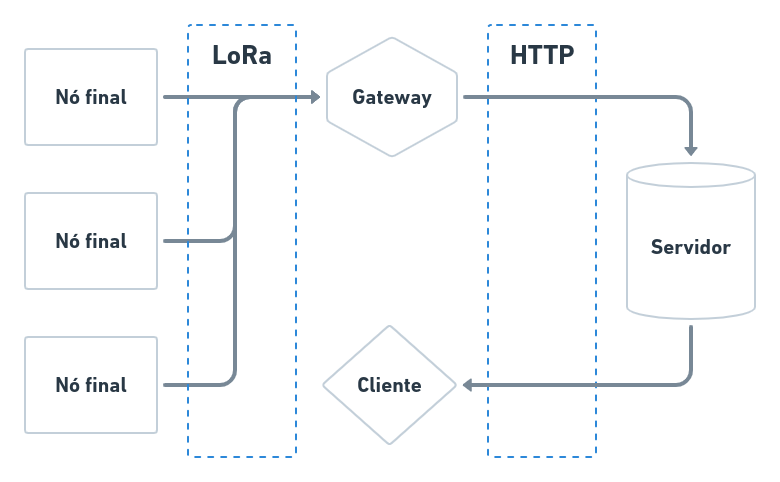
\includegraphics[width=0.4\textwidth]{assets/schematic.png}
    \end{center}
    \caption{\label{esquema} Arquitetura geral do sistema.}
    \label{fig:arch}
\end{figure}
%\subsection{Nó Final}

    Os nós finais são utilizados para obter dados coletados pelos sensores de temperatura e umidade e transmiti-los para um \textit{gateway}, por meio de  um transceptor LoRa \cite{ref2}. O fator de espalhamento (SF) do LoRa, que vai de 6 até 12\cite{ref3}, define a taxa de bits. Foi utilizado nos testes o SF igual a 7, que é o valor padrão da biblioteca usada \cite{ref4}. As camadas superiores podem ser implementadas seguindo o padrão aberto LoRaWAN entre os nós finais e o \textit{gateway}. O LoRa pode trabalhar, nas Américas, na faixa de 915~MHz \cite{ref2}. % a 928~Mhz.%, no nosso caso, optamos por usar 915~Mhz.
    
    Os nós finais utilizam o sensor DHT22 \cite{ref6} para a captação dos dados dos ambientes de armazenagem, podendo medir temperaturas entre -40$^\circ$C a 80$^\circ$C, com precisão em torno de $\pm$ 0,5$^\circ$C, e umidade de 0 a 100\%, com precisão de 0,1\%.

    O \textit{gateway} é formado por um microcontrolador com uma interface LoRa e uma interface Wi-Fi, para comunicação com os nós finais e conexão com a Internet, respectivamente. Quando ativado, ele cria um \textit{access point}, de modo que é possível se conectar para mudar as configurações de rede, se necessário, e tenta se conectar a uma rede Wi-Fi pré-configurada. Com êxito, ele recebe os dados dos nós finais, realiza a detecção de  erros  de  formato  no  pacote,  e  transmite  os  dados  para um  servidor  na  nuvem.  Essa  transmissão  para  o  servidor  é realizada através de requisições HTTP.
    
   %\rd{(O que foi usado para implementar o gateway? Como ocorre a conexão com a internet?.)}
    O servidor é responsável por armazenar os dados dos usuários, como e-mail e senha, dados dos nós finais e do \textit{gateway}, tais como identificadores e localização, além dos dados coletados pelos sensores, junto com os dados dos pacotes transmitidos pelos nós finais, como o RSSI, essencial para a realização dos testes, pois podemos analisar a qualidade dos enlaces de comunicação.
    
    O cliente é um aplicativo para Android responsável por exibir os dados coletados pelos nós finais cadastrados entre outras funções.
    %, além de permitir criar, editar e deletar os dados dos nós e dos \textit{gateways}.